\chapter{Showtime}\label{chap:Showtime}

Every semester, students of the "College of Engineering and Economic Berlin" are presenting their bachelor and master projects at a college fair called "Showtime". The event takes place at the end of each semester. Each group has 20 minutes to present their work. On this event professors and visitors have the opportunity to learn about the various projects and groups. At the same time the professors are evaluating the students' work - that is an important part of the course.

Before the "Showtime" started a lot of planning was necessary - from the actual presentation to brochures and posters. Everything needed to be planned and organized.

\section{Presentation}

The main goal of the presentation was bring our software closer to visitors and professors. 
Within the presentation the our software system on one hand was declared and shown, on the other hand substantiate with the help of theoretical foundations.

As a technical basis, we used the online presentation toll calles "impress.js", which enables similar to the Flash presentation tool "Prezi" spatial effects. With impress.js you can create individual slides which are placed in a three-dimensional space. The difference between "Prezi" and "impress.js" is the used technology of "impress.js"- CSS3 and Javascript, so you don´t have to install Adobe Flash. \footnote{http://matthiasschuetz.com/impress-js-effektvolle-zoom-praesentationen-mit-css3 - Date: 24.07.2012}.


\begin{figure}[!h]
  \centering
  \fbox{
    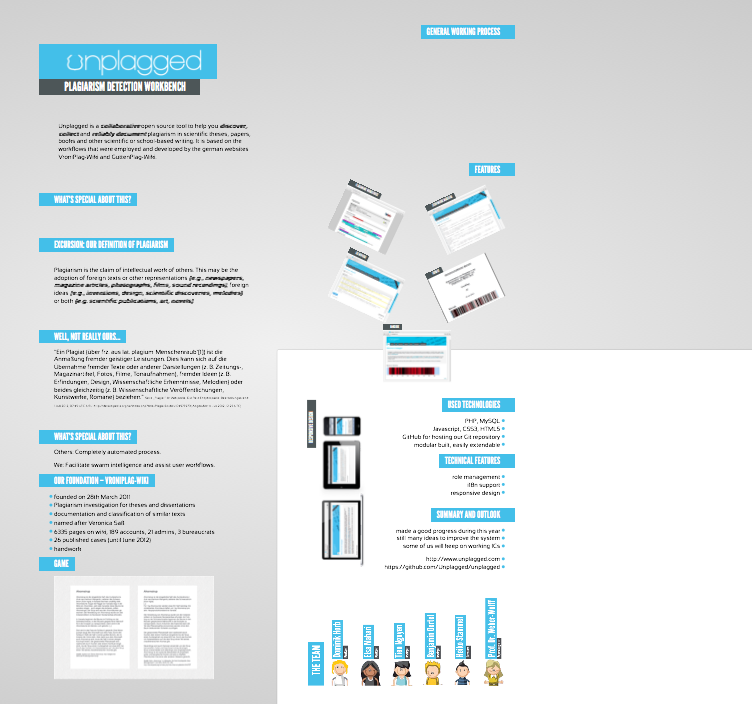
\includegraphics[width=0.97\textwidth]{images/presentation-1.png}
  }
  \caption{Our presentation in impress.js}
  \label{fig:impress.js}
\end{figure}

\subsection{Presentation sequence}
Before the start of our 20 minute presentation, we distributed handouts and pens. These handouts two different texts: On the left the plagiarism candidate to the right the source from Wikipedia.
After we had introduced to ourselves, one of the students led to the presentation. He explained the meaning and purpose of our software and the advantages and differences compared to competitors. Afterwards another group member gave an overview of the history and work of our client "Vroniplag". 
In the third part a group member entered into the handouts, to explain the visitors and professors what it was all about the game. It was about to clarify the difficulties and the effort in the finding process of plagiarism - the daily bread of our professor. For this purpose the visitors had to compare the two texts of the handout and highlight any similarities with the pen. Of course, 50 percent of the text were plagiarized.
Then our six-minute film was shown. The film explains the functionality of our software. 
After the audience had gained a glimpse into the software, another group member explained the features of the software in detail. After this we explained, which technologies were used to create the software. Finally, we ventured a look into the future of "Unplagged", lets say we designed future plans for the software.


\begin{figure}[!h]
  \centering
  \fbox{
    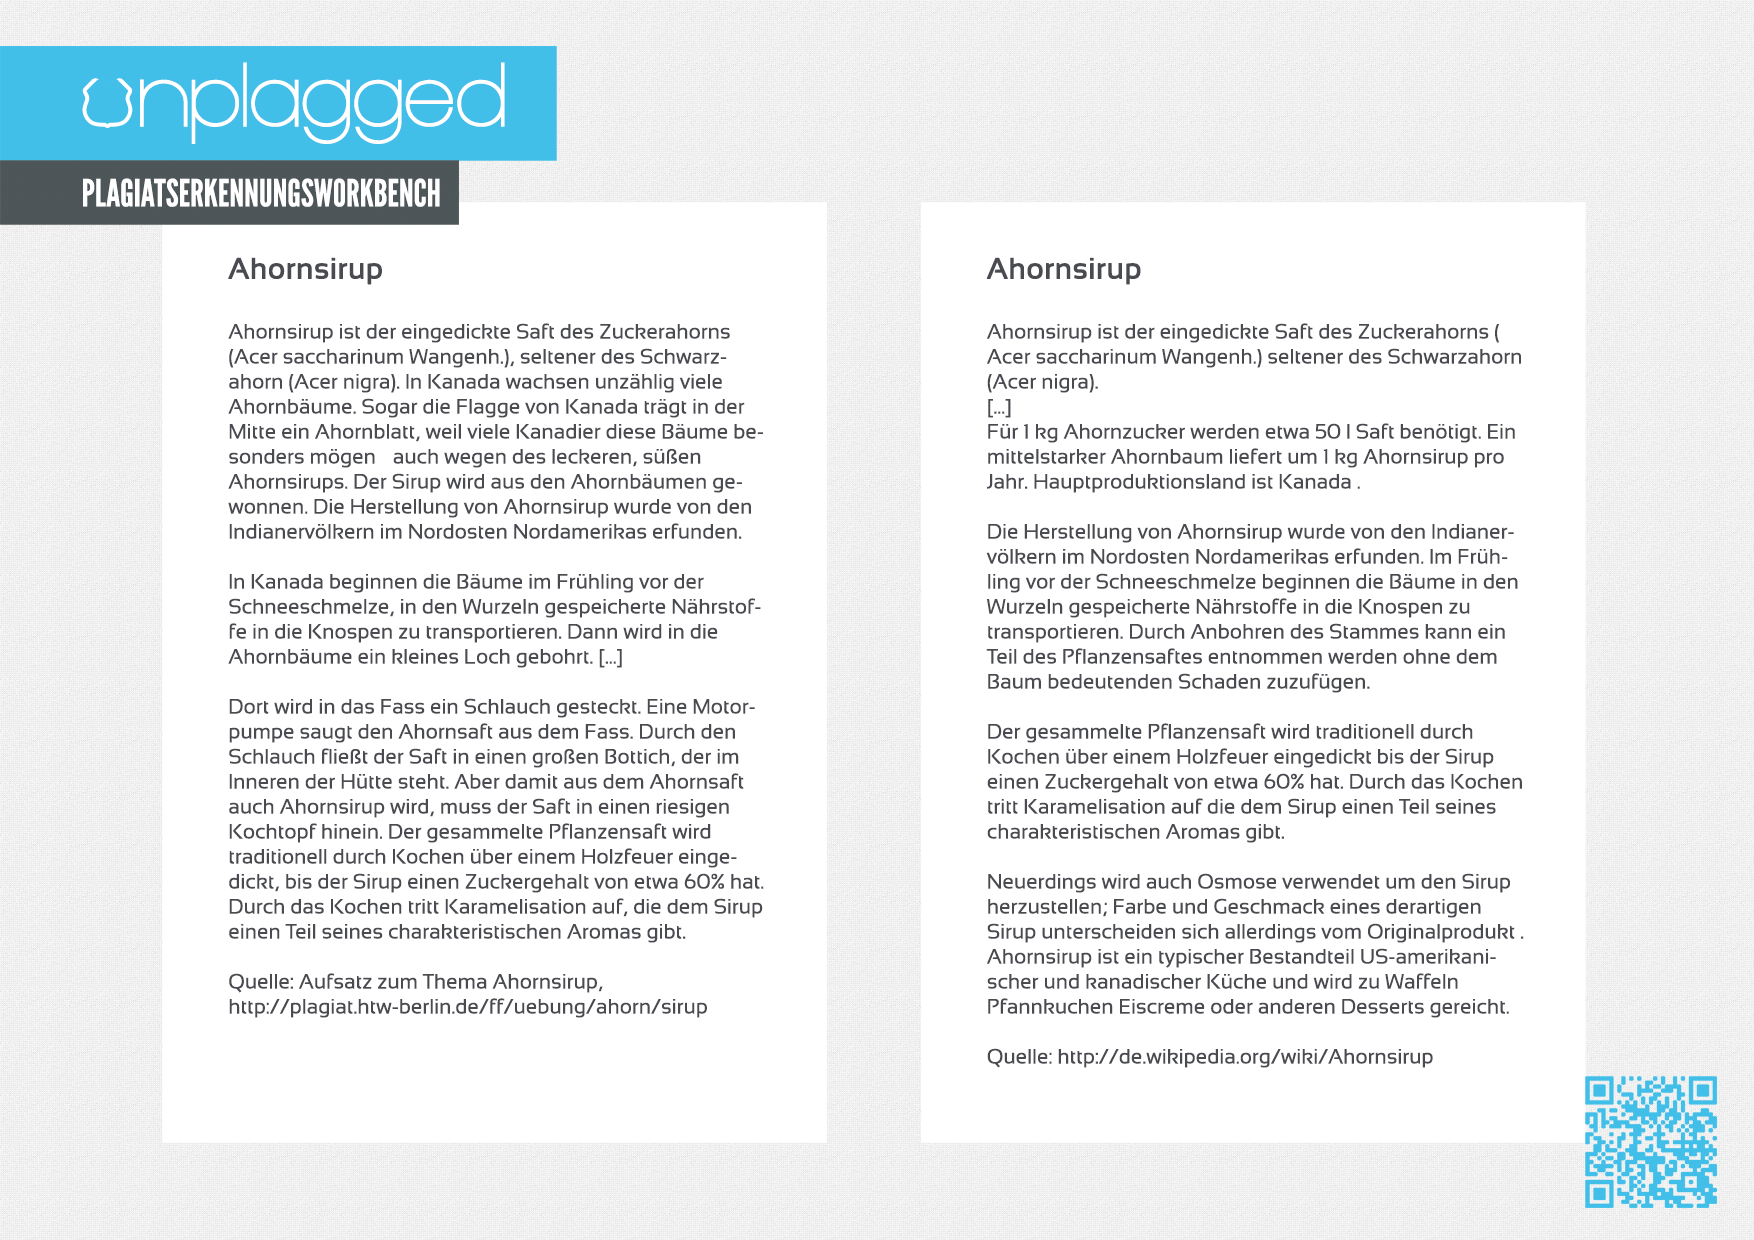
\includegraphics[width=0.97\textwidth]{images/game_handout.png}
  }
  \caption{Game Handout}
  \label{fig:game-handout}
\end{figure}



\subsection{Presentation movie}
The aim of the film was on the one hand to make the software even understandable for laymen, on the other hand to loosen the presentation. The film consisted of animations, which suggested the spectator would himself use the software and analyze a document for plagiarism. Additionally the presentation of the film was shown continuously at the booth.

\begin{figure}[!h]
  \centering
  \fbox{
    
\includegraphics[width=0.5\textwidth]{images/descriptive-headline.png}
  }
  \caption{Movie descriptive headline}
  \label{fig:descriptive-headline}
\end{figure}


\pagebreak 


\subsection{Movie creation}
For film production, we used Adobe After Effects and Adobe Photoshop. The film showed the chronological order of the plagiarism process. This works best for the spectator when he sees the screen, he would also actually see before them. Each new scene was launched with a descriptive headline. After this we used a screencast software to show how to log in, upload documents, searches for plagiarism, divides into fragments, creating documents and automated comparing of documents- in short, how the software works. The mouse cursor was marked for greater clarity in color constantly. Instead of a rigid voice-over, we let a group member to take the voice-over. So we were able to respond optimally to questions of the audience.


\begin{figure}[!hbtp]
  \centering
  \fbox{
    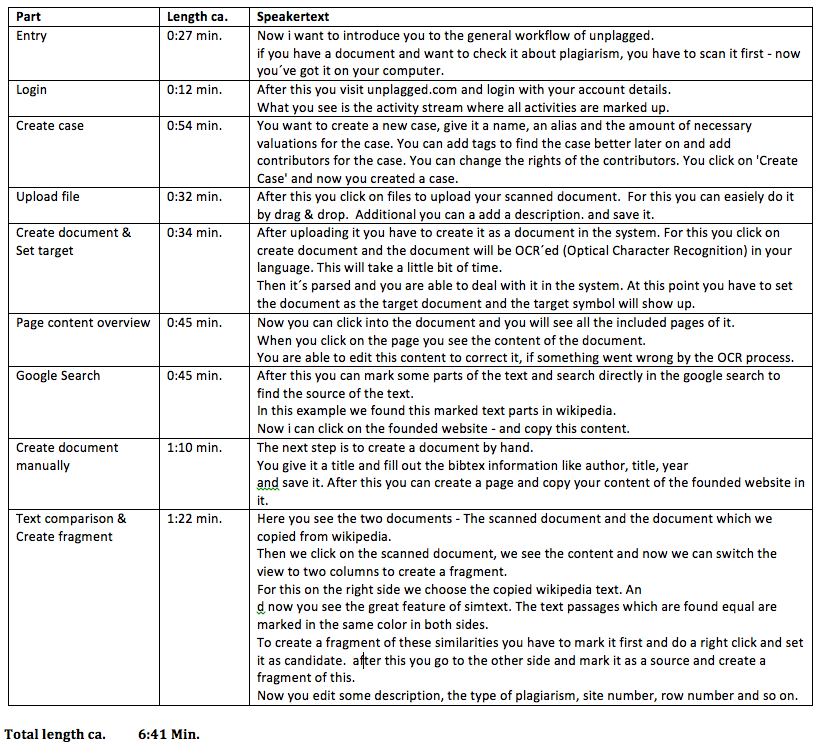
\includegraphics[width=1\textwidth]{images/movie-parts.png}
  }
  \caption{Presentation movie structure}
  \label{fig:fpresentation-movie-structure}
\end{figure}

\begin{figure}[!hbtp]
  \centering
  \fbox{
    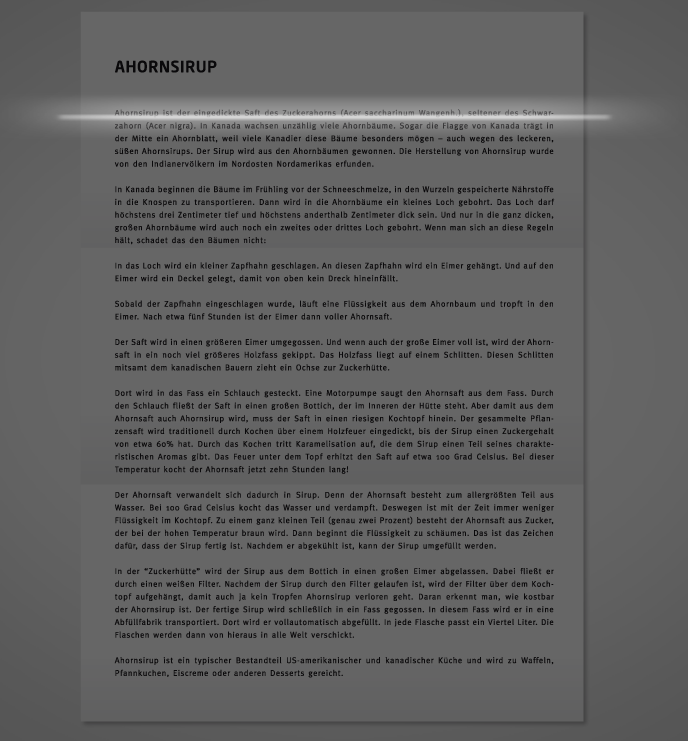
\includegraphics[width=0.5\textwidth]{images/scan-animation.png}
  }
  \caption{Scan Animation}
  \label{fig:scan-animation}
\end{figure}

\begin{figure}[!hbtp]
  \centering
  \fbox{
    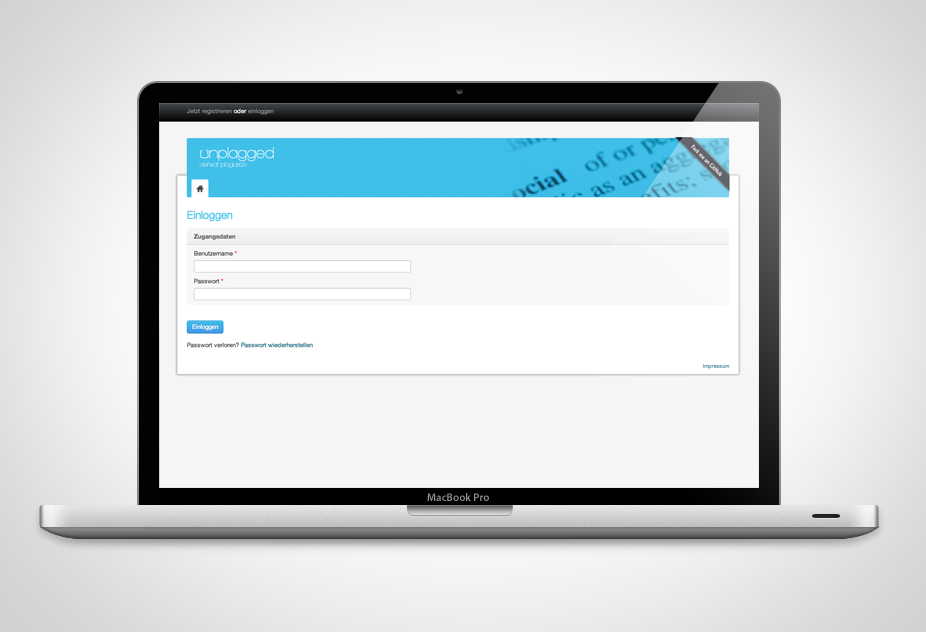
\includegraphics[width=0.5\textwidth]{images/macbook.png}
  }
  \caption{Macbook animation}
  \label{fig:macbook}
\end{figure}

\pagebreak 


\section{Paperwork}
At the beginning it was necessary to make a first concept of the brochure and posters for the unplagged exhibition stand.

\subsection{Brochure}


In addition to various posters, we developed a two-page brochure. The lay out of the booth and could be freely taken by the visitors. It gave a brief outline of our project and the visitors had the opportunity to call back the most important points into memory.
This was the first concept of the brochure, which was kind of a sketch.





\begin{figure}[!hbtp]
  \centering
  \fbox{
    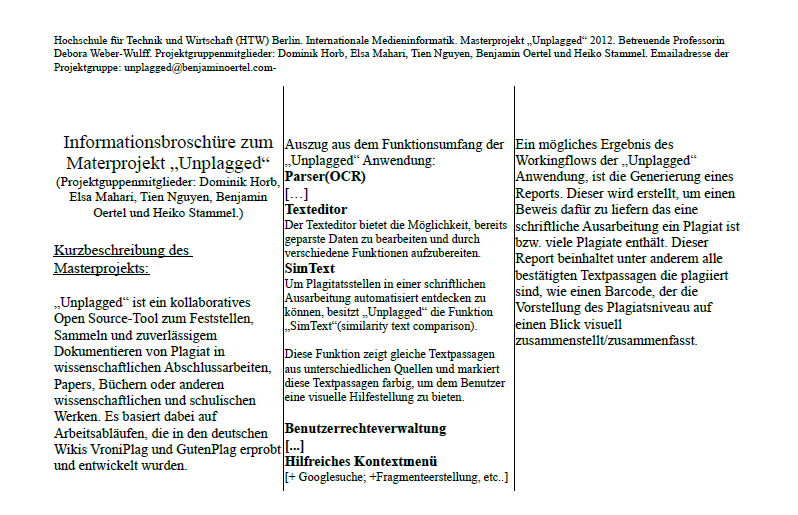
\includegraphics[width=0.97\textwidth]{images/brochure_sketch.png}
  }
  \caption{the first concept of the brochure}
  \label{fig:brochure_sketch}
\end{figure}

Below is the final outlook of the brochure.

\begin{figure}[!hbtp]
  \centering
  \fbox{
    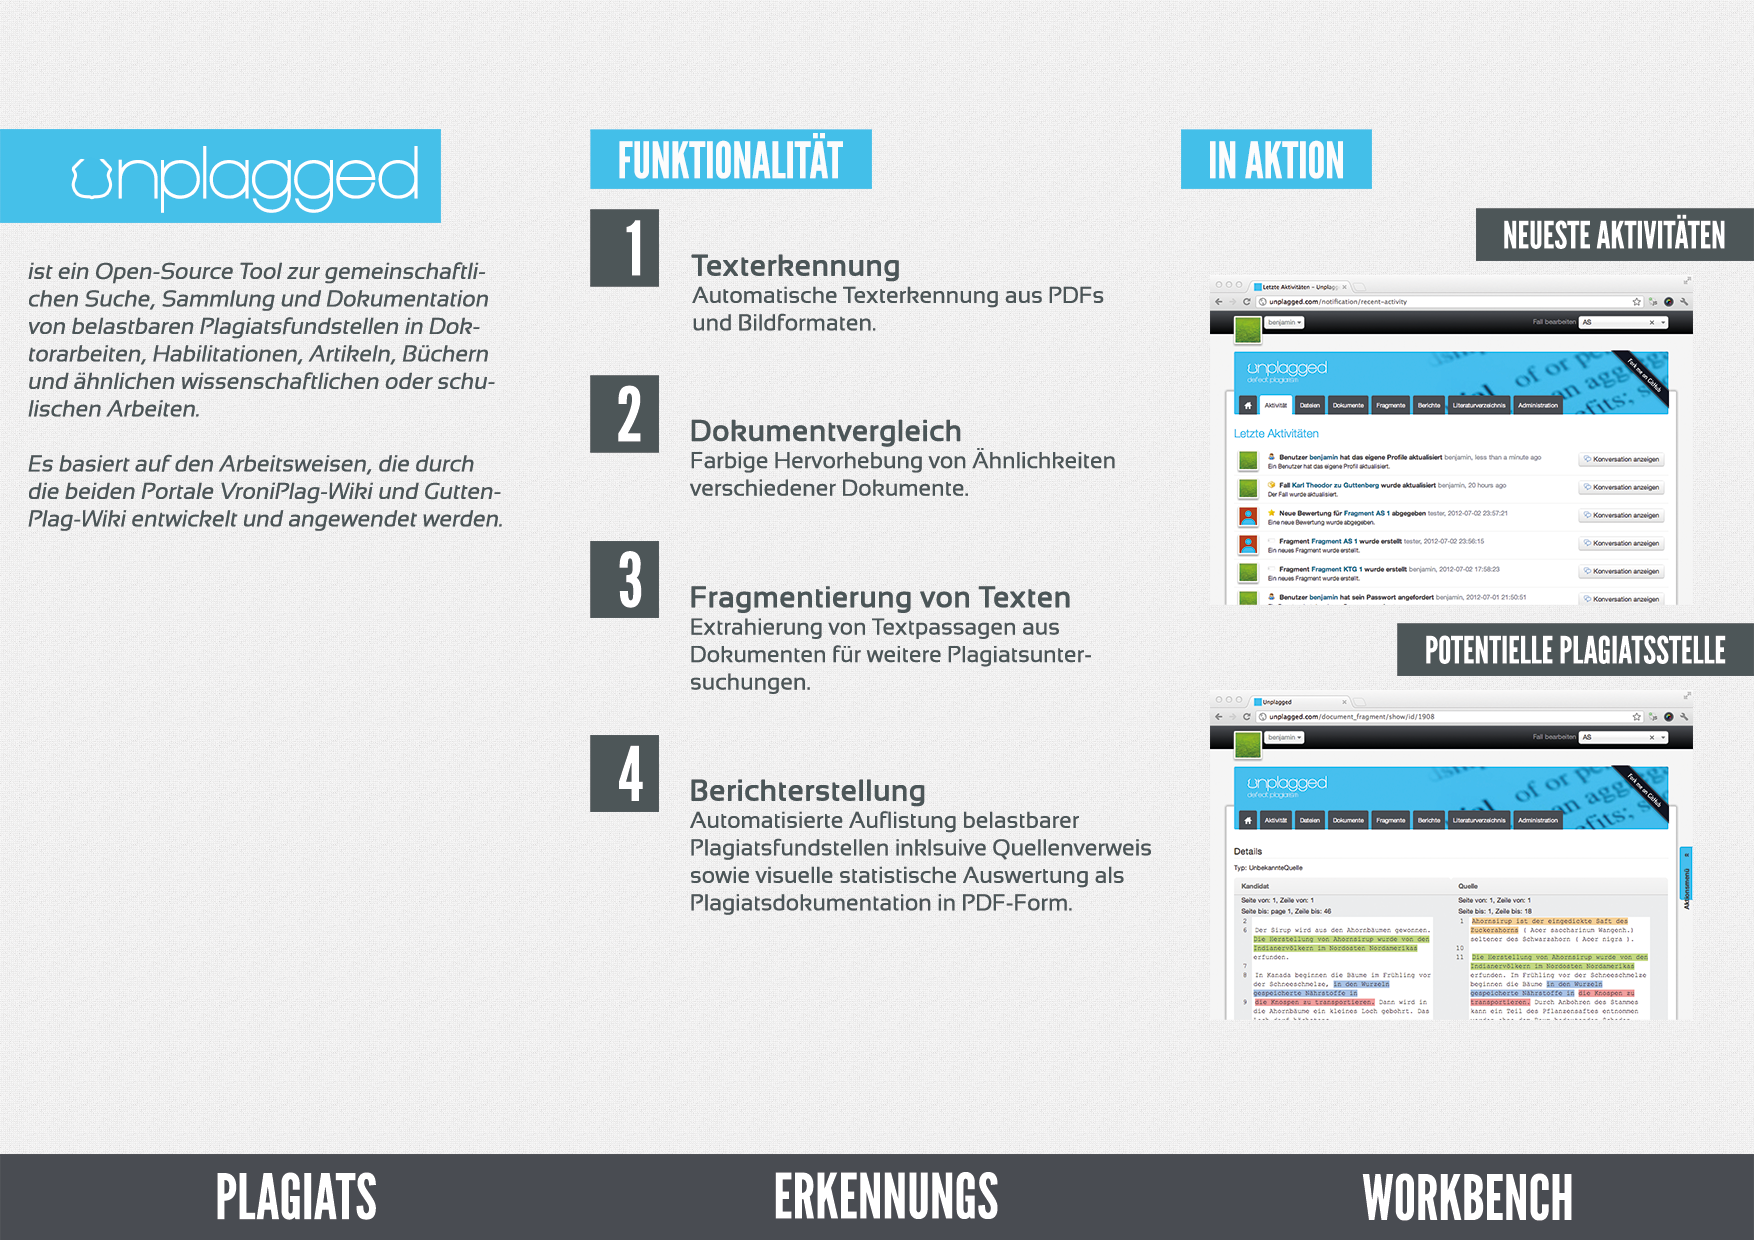
\includegraphics[width=0.97\textwidth]{images/a4_tri-fold_inside.png}
  }
  \caption{the frontside of the final unplagged brochure}
  \label{fig:brochure_final_frontside}
\end{figure}

\begin{figure}[!hbtp]
  \centering
  \fbox{
    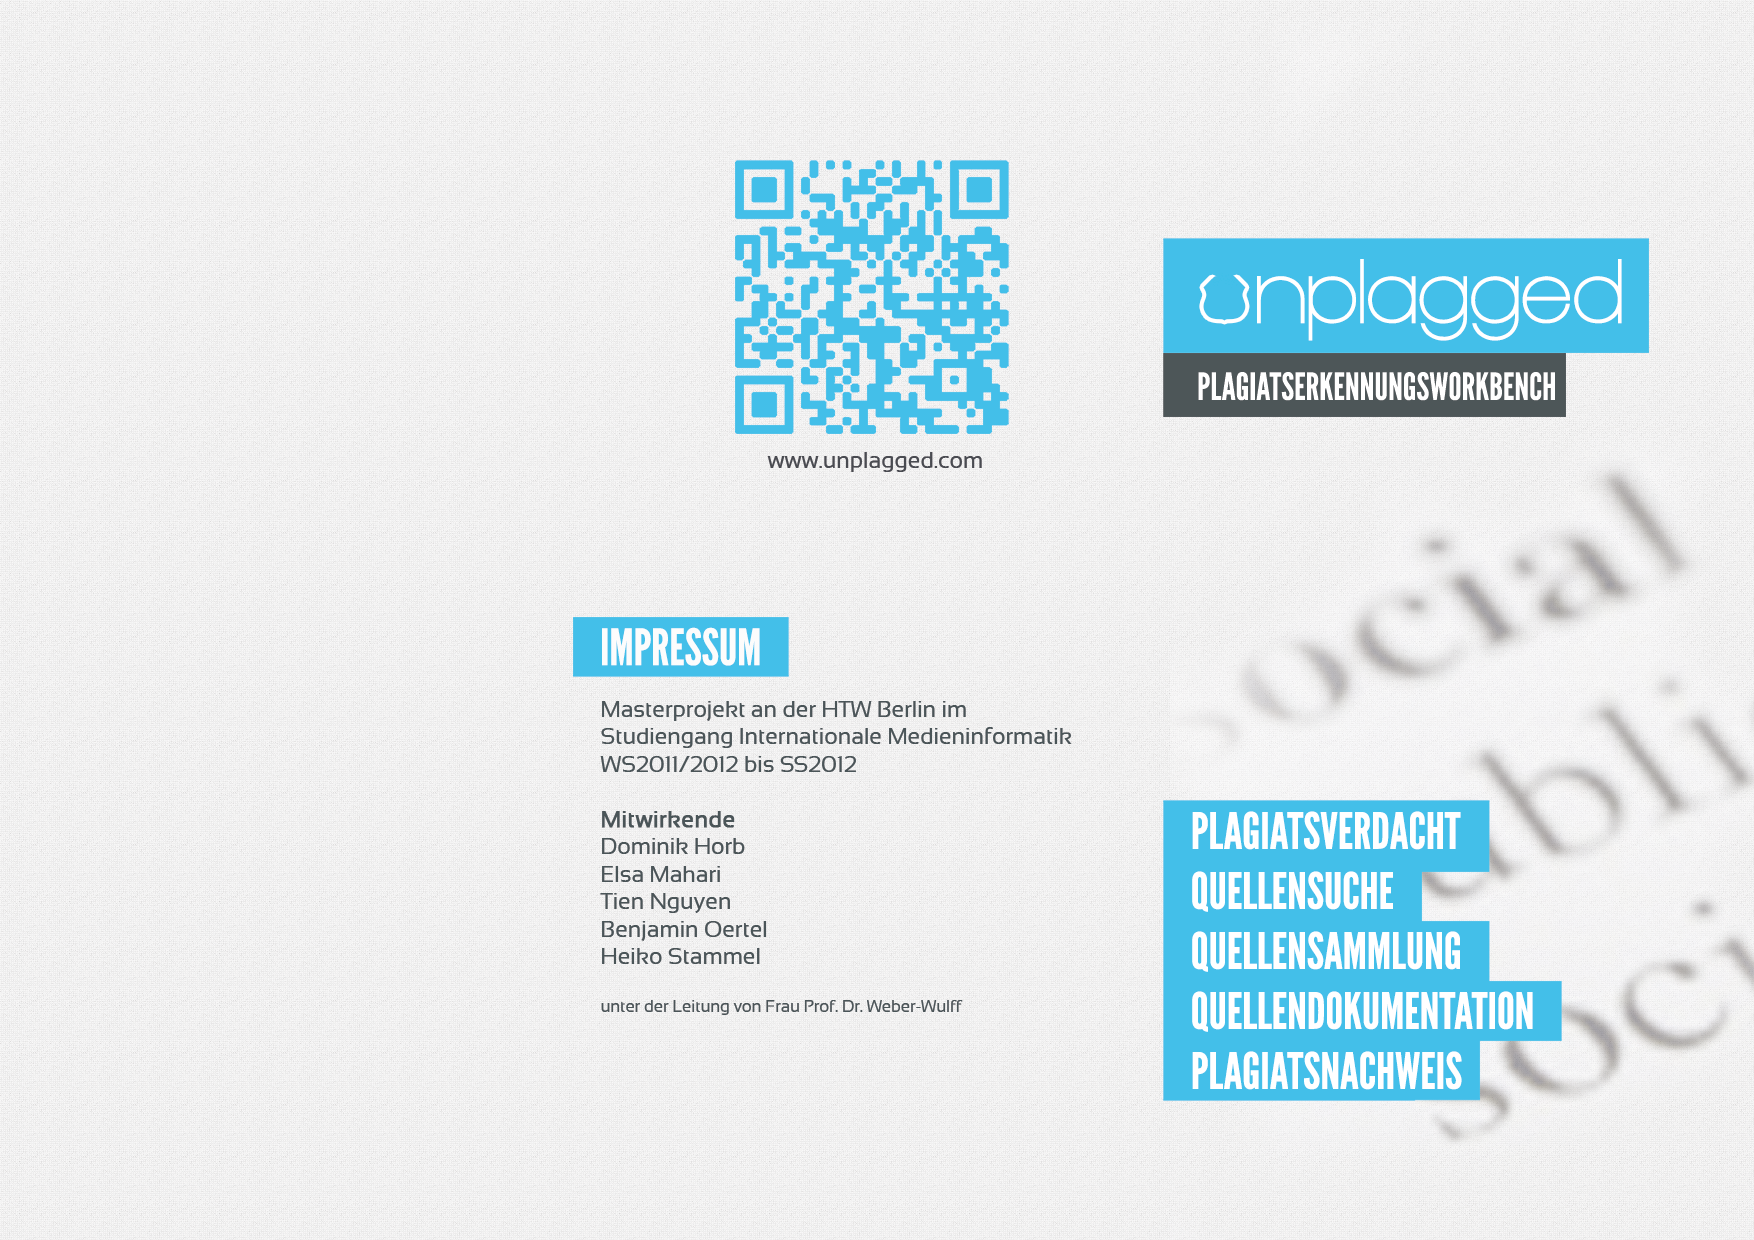
\includegraphics[width=0.97\textwidth]{images/a4_tri-fold_outside.png}
  }
  \caption{the backside of the final unplagged brochure}
  \label{fig:brochure_final_backside}
\end{figure}

\pagebreak 

\subsection{Posters}

The posters were developed mainly for the booth. Visitors and professors could thus provide a first quick overview about our project. At the same time they were supposed to generate attention: 
A technical Poster which gave the visitors an overview about the technology we used, 
a team poster with a survey about the team members, the key features, a programming sprint overview and a poster with the "Unplugged" logo.


\subsubsection{Title Poster}

\begin{figure}[!hbtp]
  \centering
  \fbox{
    
\includegraphics[width=0.97\textwidth]{images/a4_logo.png}
  }
  \caption{the title poster}
  \label{fig:poster_title}
\end{figure}

\pagebreak

\subsubsection{Describing Poster}

\begin{figure}[!hbtp]
  \centering
  \fbox{
    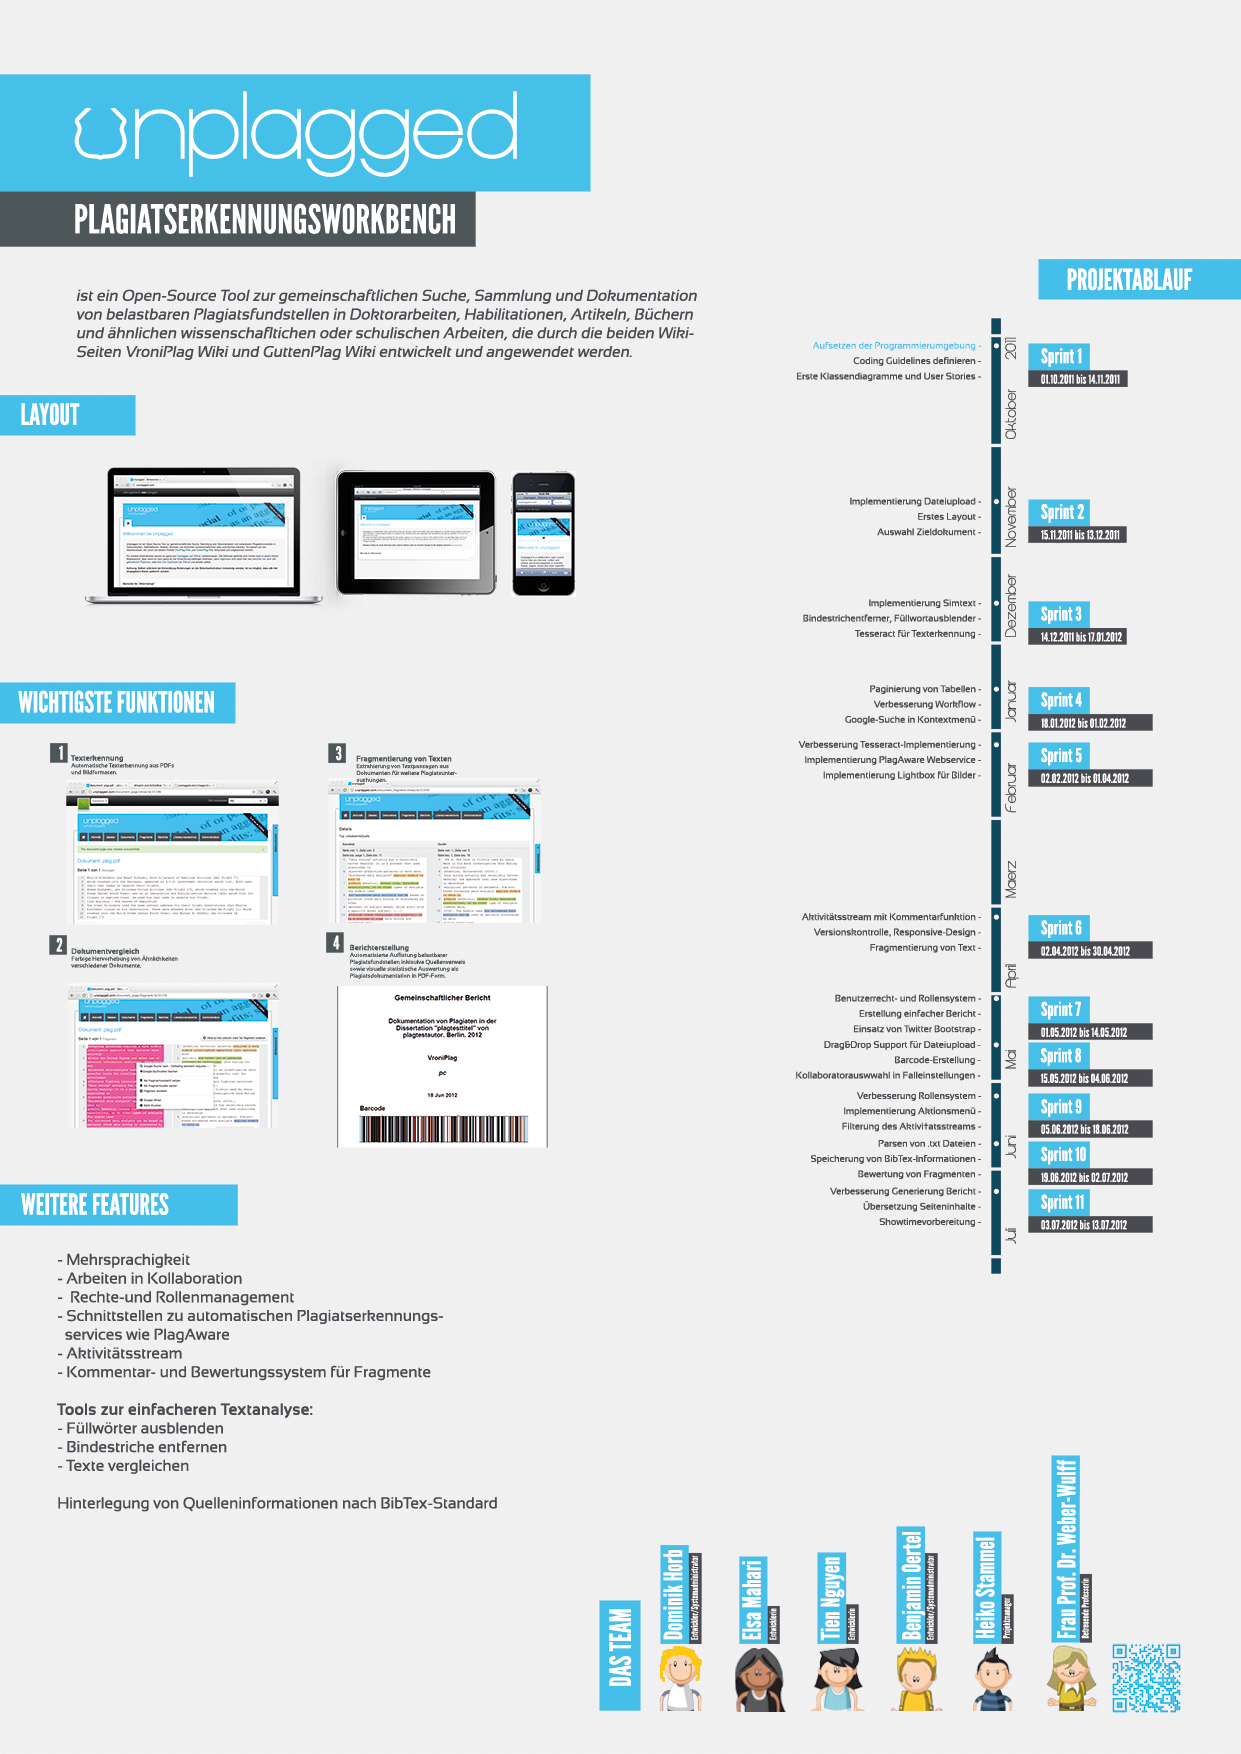
\includegraphics[width=0.8\textwidth]{images/a4_poster_general.png}
  }
  \caption{the describing poster}
  \label{fig:poster_describing}
\end{figure}

\pagebreak

\subsubsection{Technical Poster}

Below is a cutout of the technical poster.

\begin{figure}[!hbtp]
  \centering
  \fbox{
    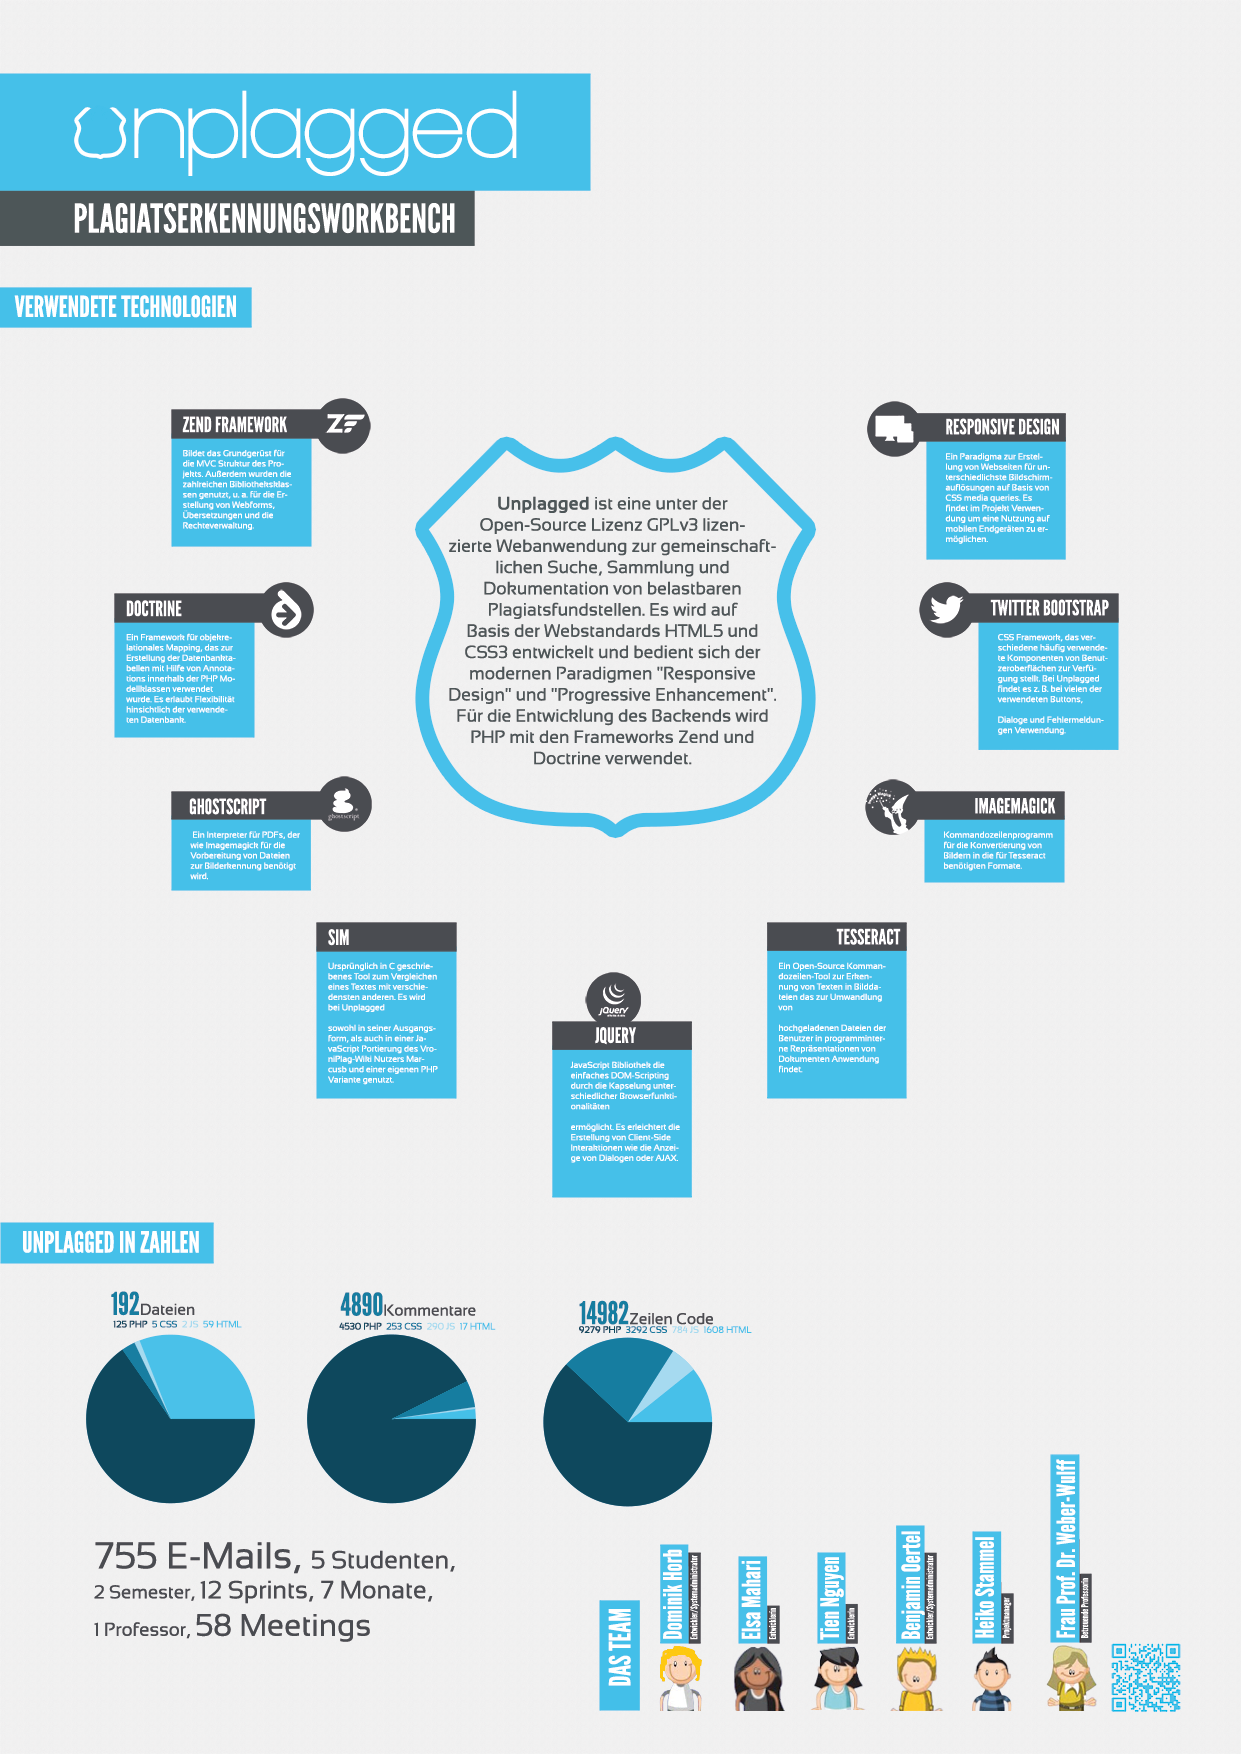
\includegraphics[width=0.8\textwidth]{images/a4_poster_technology.png}
  }
  \caption{the technical poster}
  \label{fig:poster_technical}
\end{figure}

\pagebreak 


\section{Exhibition stand}

The best possible way to present our software was to hang three posters in the background. 



\begin{figure}[!hbtp]
  \centering
  \fbox{
    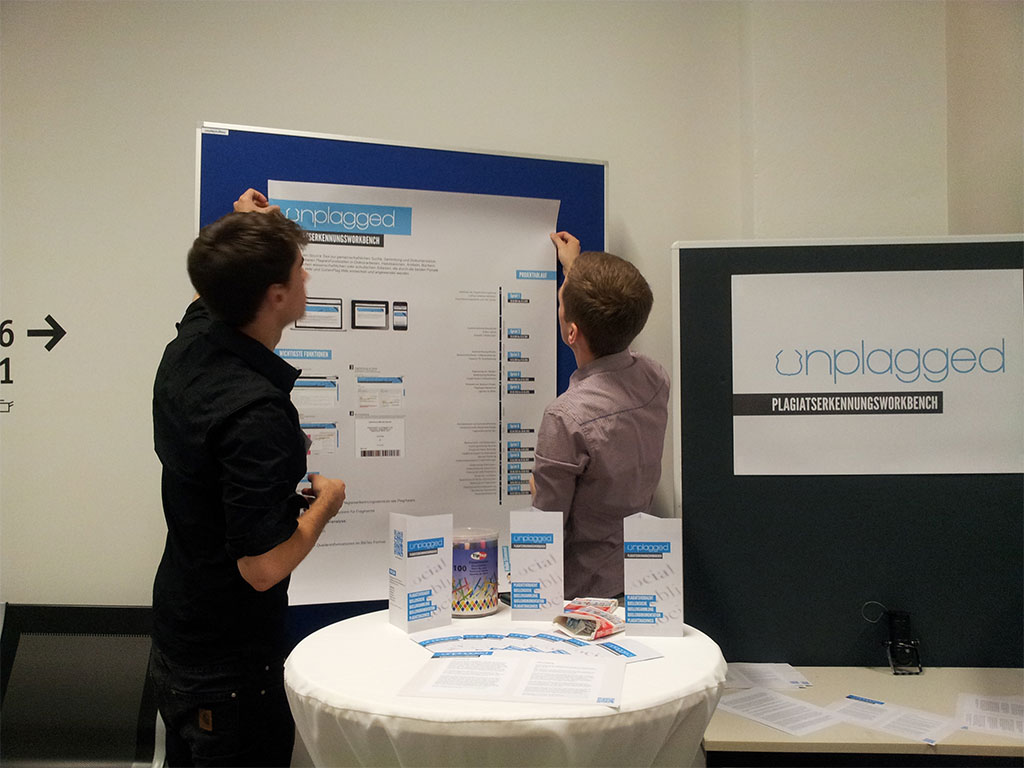
\includegraphics[width=0.97\textwidth]{images/unplagged_exhibition_stand1.jpg}
  }
  \caption{unplagged exhibition stand}
  \label{fig:unplagged_exhibition_stand1}
\end{figure}

\pagebreak

The stand itself was equipped with three iMacs to be able demonstrate the software.
Once a computer was idle, we let the film run on the desktop.
Additionally, we distributed the brochure with a brief over view About "Unplugged".
The whole day we were about to answer visitors' questions, the offer has been widely used.
Below there are some snapshots of the unplagged exhibition stand.

\begin{figure}[!hbtp]
  \centering
  \fbox{
    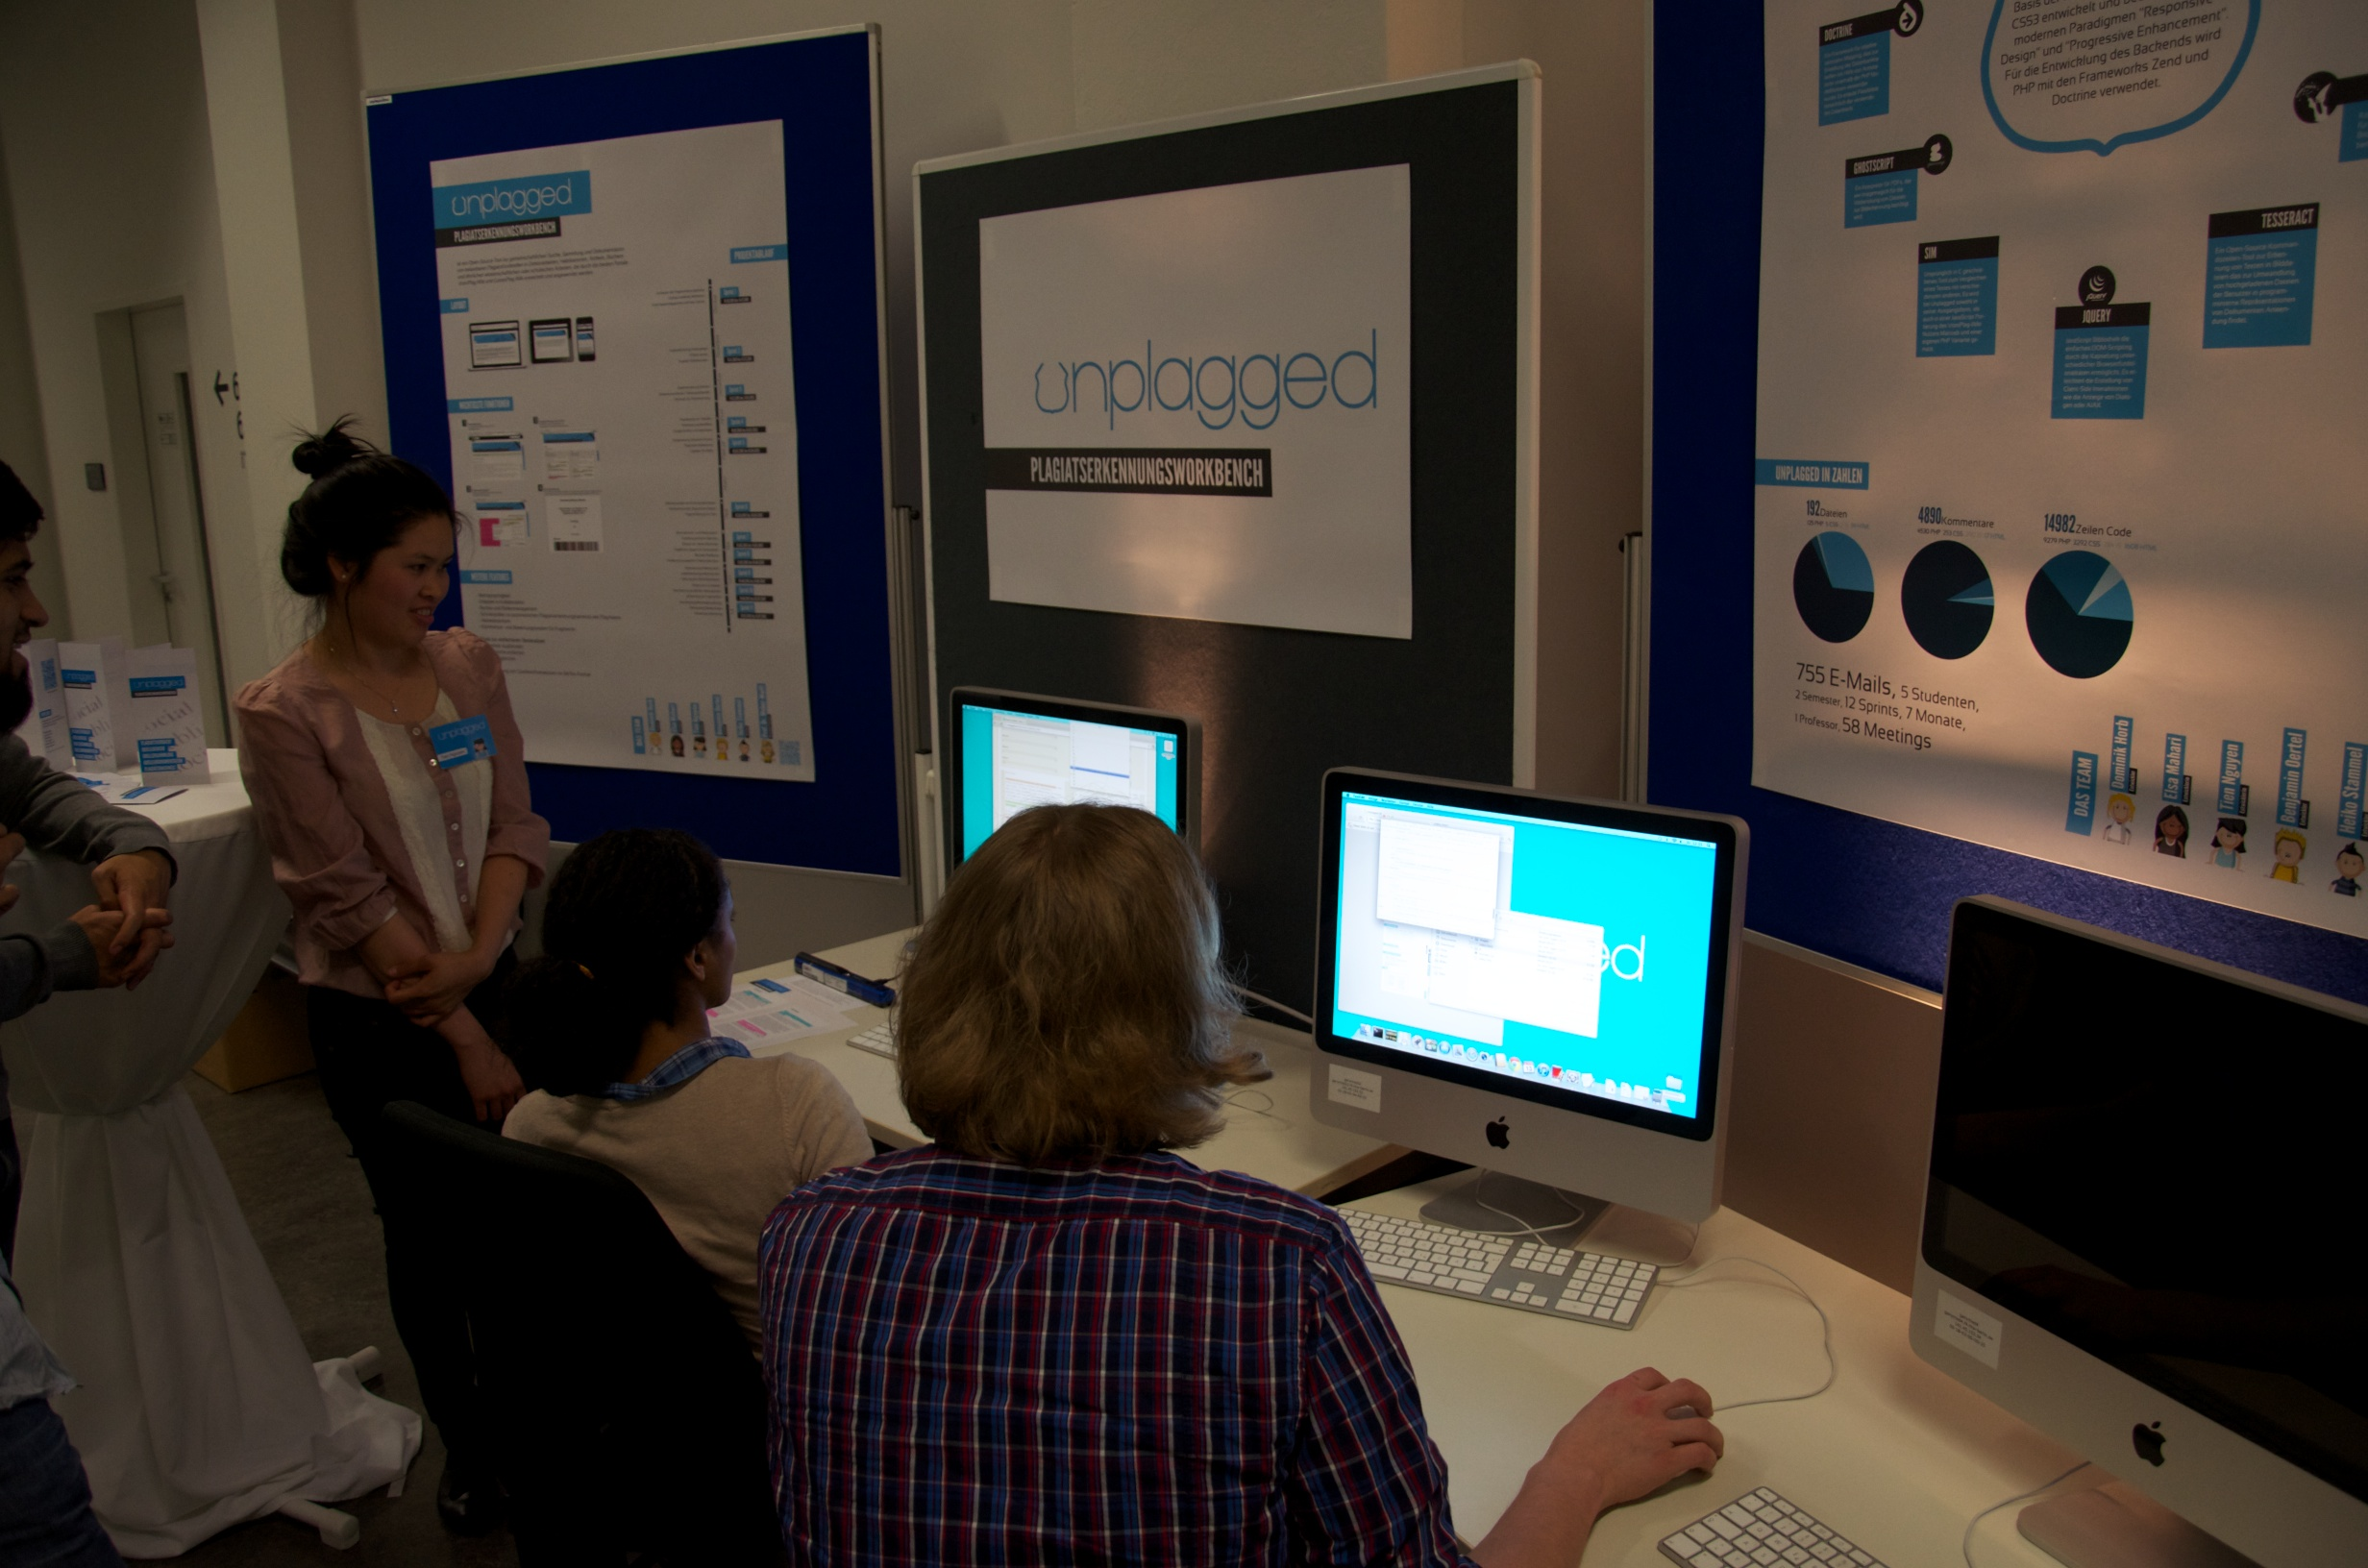
\includegraphics[width=0.97\textwidth]{images/DSC_0173.jpg}
  }
  \caption{unplagged exhibition stand}
  \label{fig:unplagged_exhibition_stand2}
\end{figure}

\pagebreak 

\begin{figure}[!hbtp]
  \centering
  \fbox{
    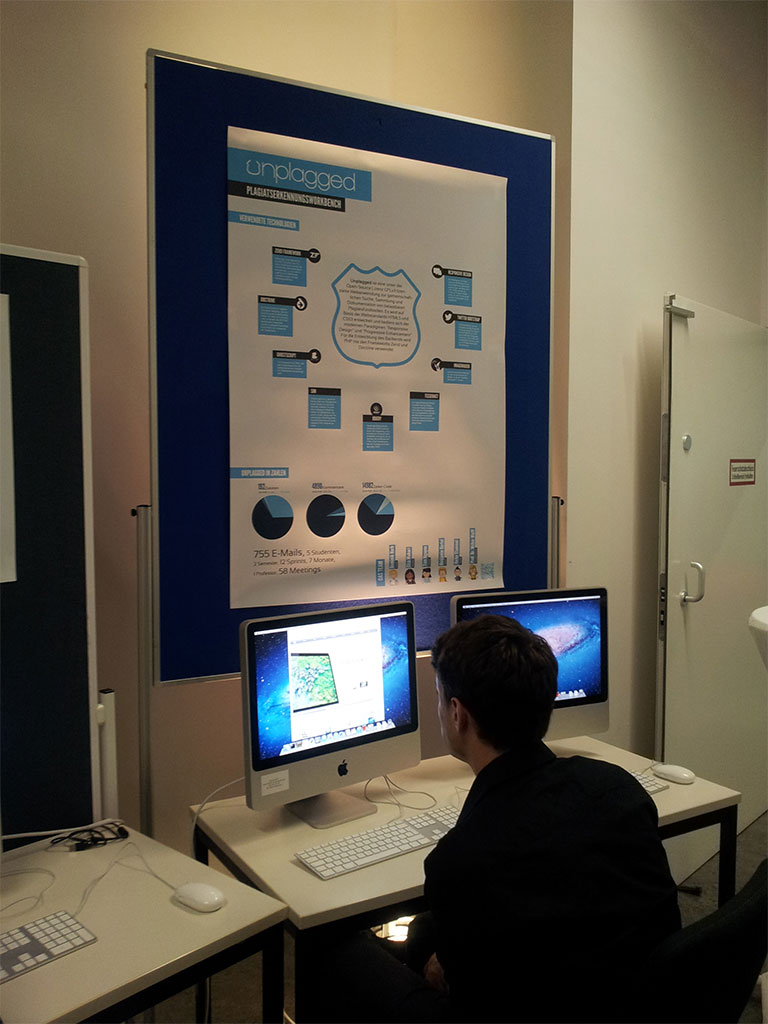
\includegraphics[width=0.97\textwidth]{images/unplagged_exhibition_stand3.jpg}
  }
  \caption{unplagged exhibition stand}
  \label{fig:unplagged_exhibition_stand3}
\end{figure}

\pagebreak

\begin{figure}[!hbtp]
  \centering
  \fbox{
    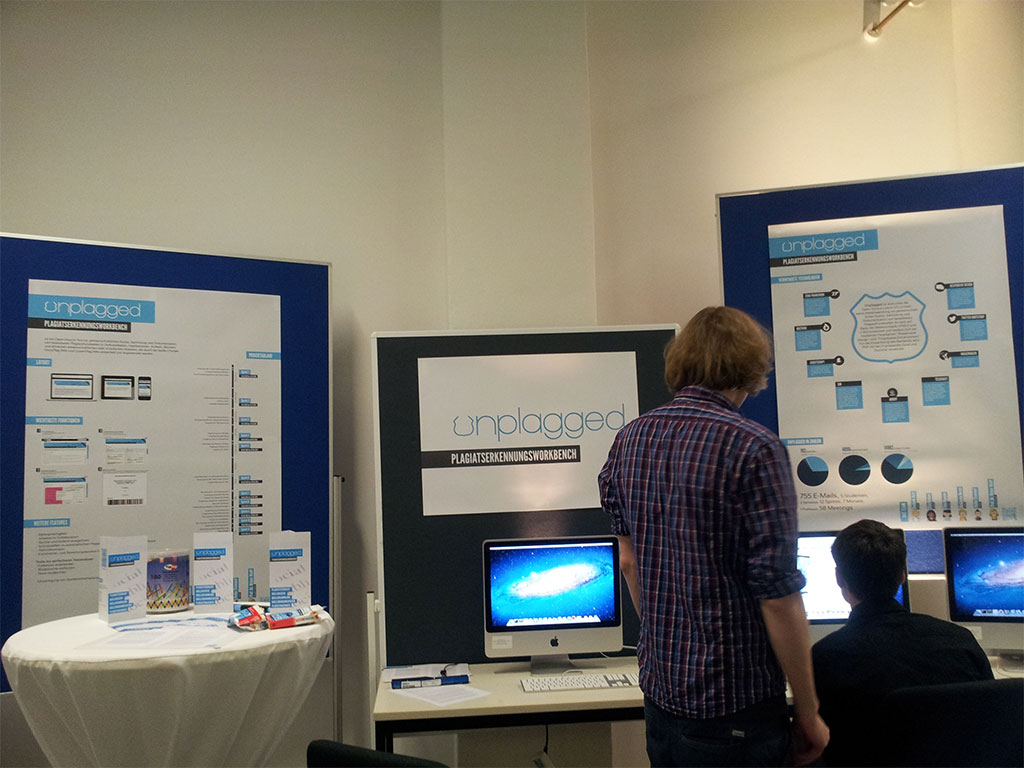
\includegraphics[width=0.97\textwidth]{images/unplagged_exhibition_stand4.jpg}
  }
  \caption{unplagged exhibition stand}
  \label{fig:unplagged_exhibition_stand4}
\end{figure}

\pagebreak

\begin{figure}[!hbtp]
  \centering
  \fbox{
    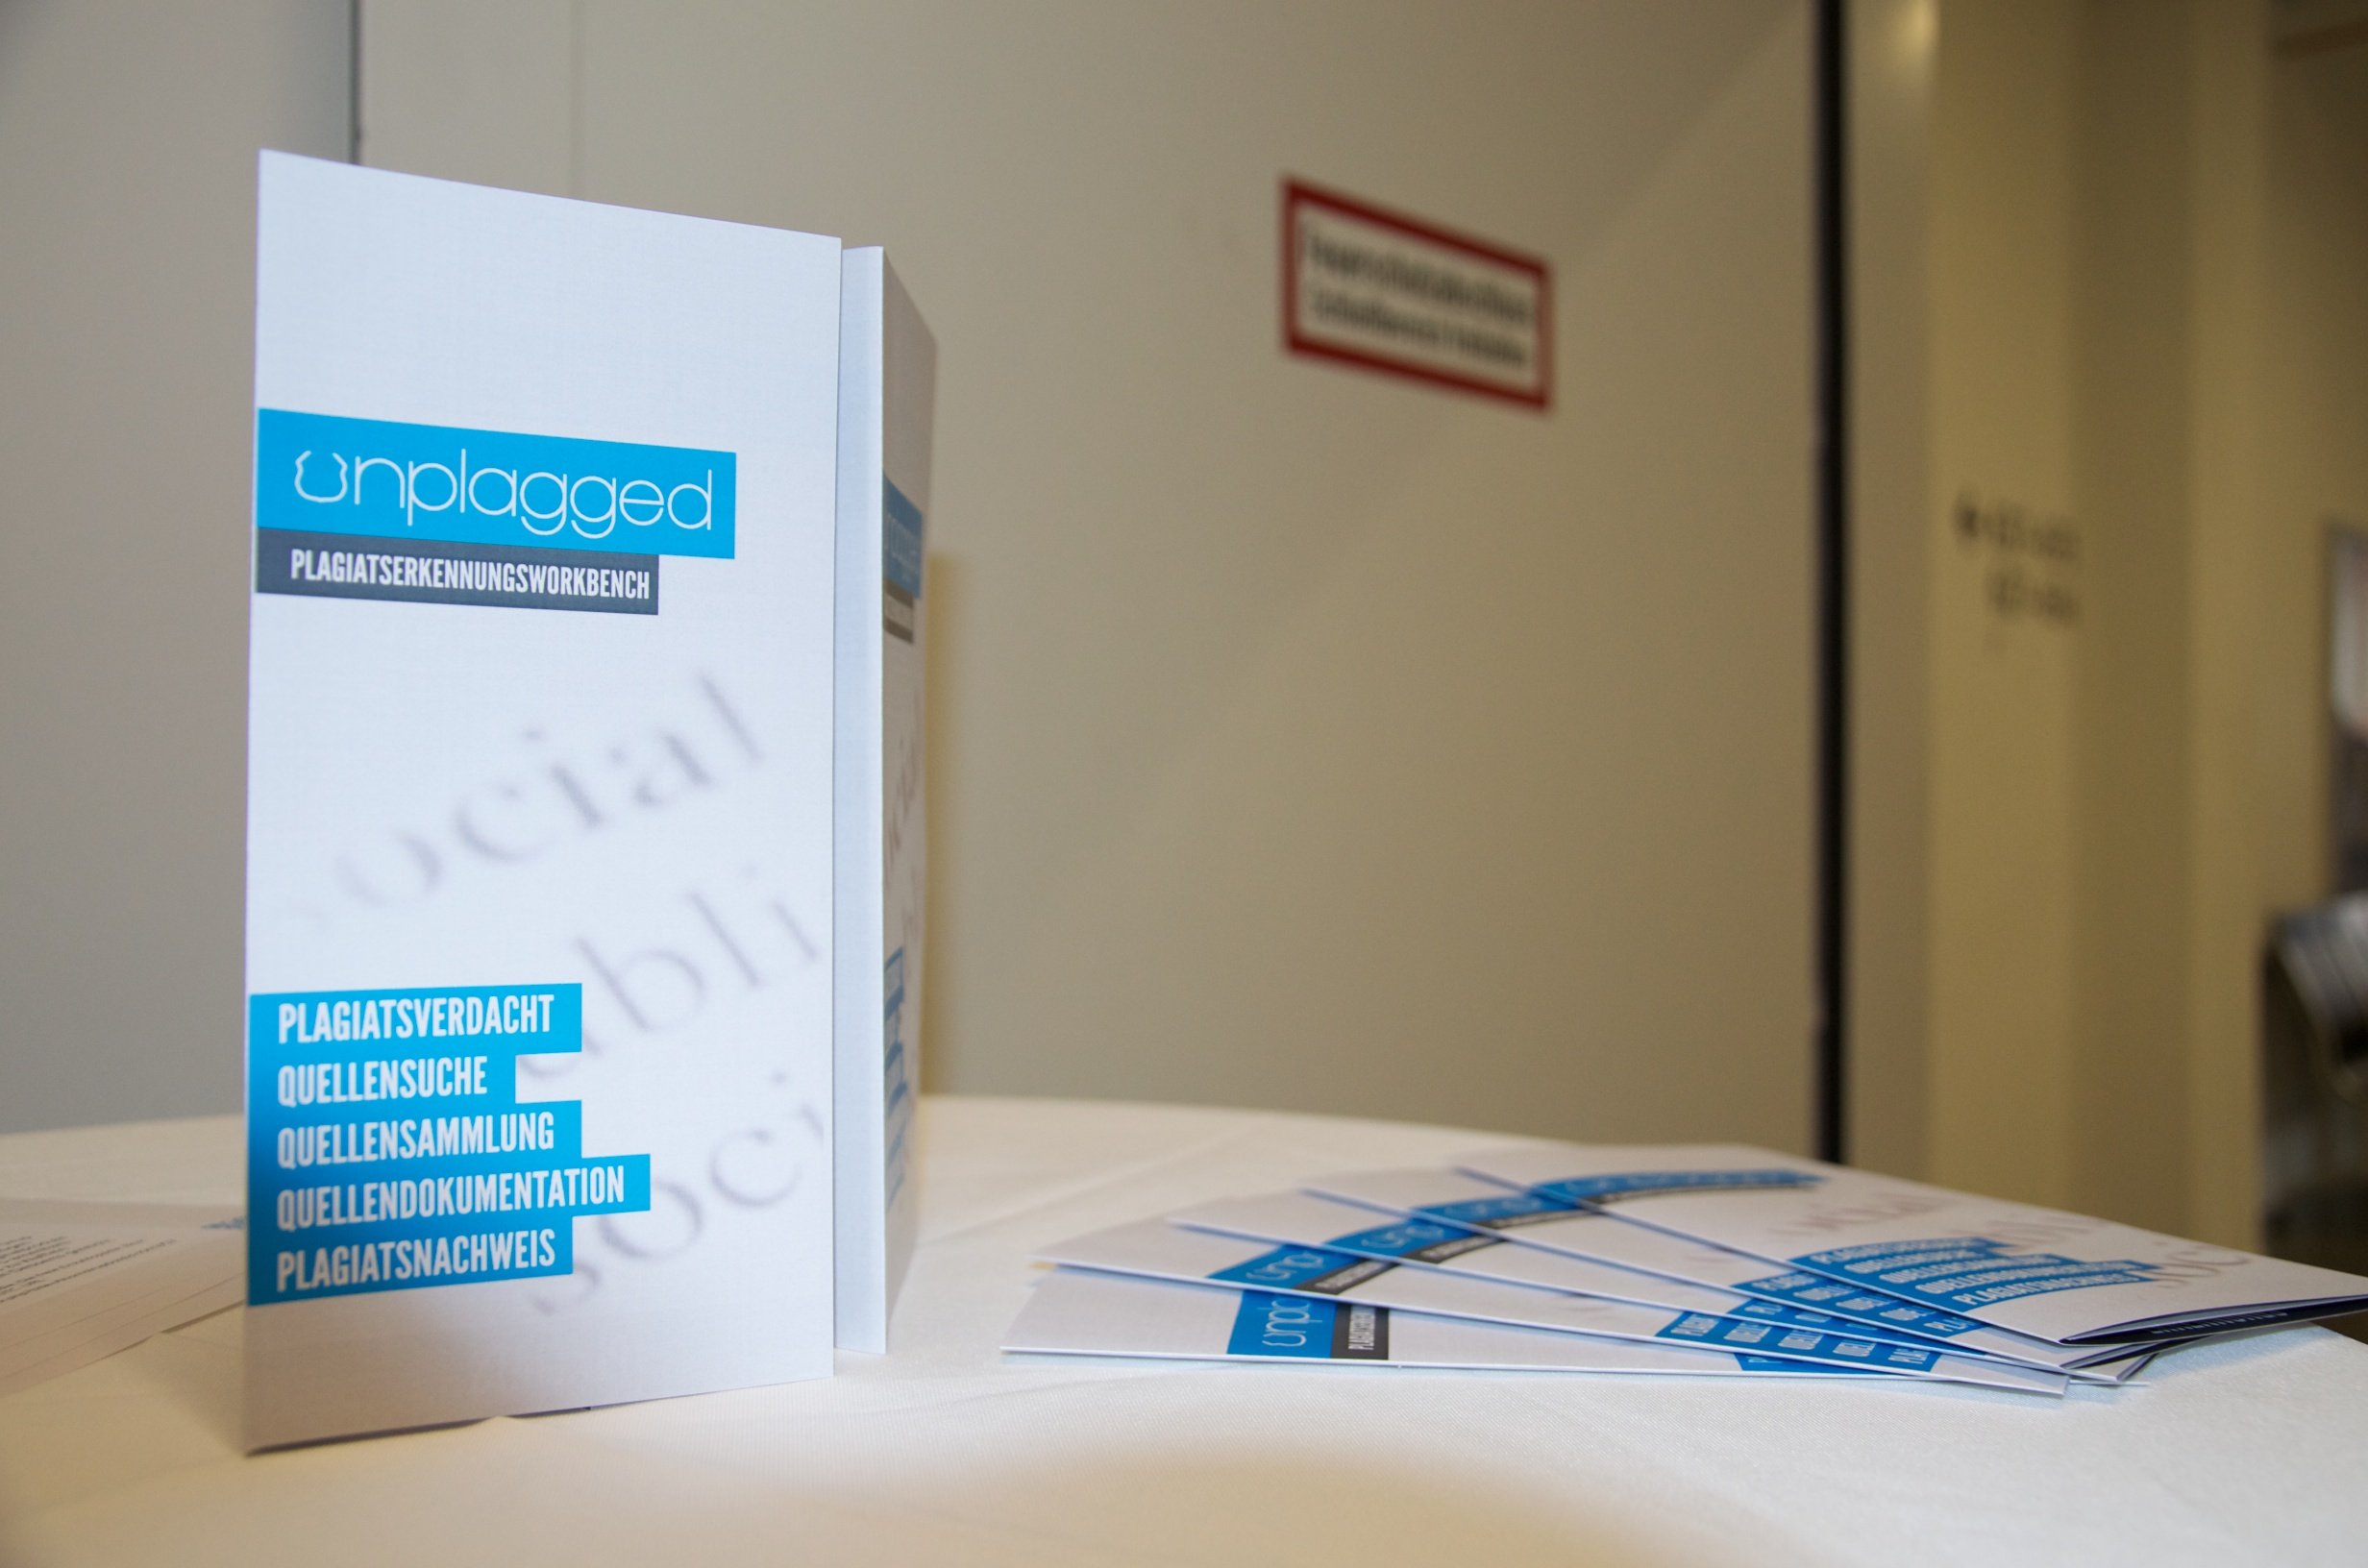
\includegraphics[width=0.97\textwidth]{images/DSC_0162.jpg}
  }
  \caption{unplagged exhibition stand}
  \label{fig:unplagged_exhibition_stand4}
\end{figure}

\pagebreak